%!TEX root = adventure.tex

\section*{Abenteuerspezifische Informationen}
% Spezielle Regeln des Abenteuers

In diesem Abenteuer erleben die Spielerinnen und Spieler den Ausbruch der Pest in der
mittelalterlichen Handelsmetropole Hamburg. Es gilt herauszufinden, was genau es mit
dem schwarzen Tod auf sich hat, wie die Stadt vor dem Unheil beschützt werden kann,
und vielleicht sogar, wie man Erkrankte wieder heilen kann. Wie sich herausstelt ein
Tanz auf Messers Schneide, denn die Krankheit macht auch vor den Spielern nicht halt.

\subsection*{Regelwerk}
\label{ssec:rules}

\definecolor{darkgreen}{RGB}{0,100,0}
\newcommand{\Pestilenz}[1][]{\textbf{\textcolor{darkgreen}{Pestilenz\ifthenelse{\equal{#1}{}}{}{$\;#1$}}}}

Ein wichtiges Element dieses Abenteuers ist die Tatsache, dass Spielcharaktere im
Verlauf der Handlung mit der Pest in Berührung treten. Sind sie dabei fahrlässig
kann es passieren, dass sie selbst an der Pest erkranken. Hierzu wurde die
\Pestilenz{}$\,$implementiert, die den Fortschritt einer Pestinfektion in Zahlen
fasst. Die Spieler sollen davon jedoch nichts mitkriegen. Lediglich Symptone der
Infektion treten auf, wenn ein Spieler einen gewissen \Pestilenz{}-Wert
überschreitet.

\begin{center}
\begingroup
\renewcommand{\arraystretch}{1.4}
  \begin{tabular*}{0.8\textwidth}{@{\extracolsep{\fill}} lr}
    \toprule
    Anzahl & Auswirkung \\
    \midrule
    \Pestilenz[1-2] & Schwindel und leichte Gleichgewichtsstörungen \\
    \Pestilenz[3-4] & Schüttelfrost und leichte Gliederschmerzen \\
    \Pestilenz[5-6] & Kopfschmerzen, Sehbeschwerden und Fieber \\
    \Pestilenz[7-8] & andere Leute merken, dass der Spieler krank ist \\
    \Pestilenz[9-10] & eitrige Beulen treten unter den Achseln auf \\
    \Pestilenz[>10] & strenge Bettlägerigkeit, der Tod folg bald \\
    \bottomrule
  \end{tabular*}
\endgroup
\end{center}

\newcommand{\Moral}[1][]{\textbf{\textcolor{darkgreen}{Moral\ifthenelse{\equal{#1}{}}{}{$\;(#1)$}}}}

Der Erfolg der Gruppe ist schwer zu quantisieren. Um dem Spielleiter dabei zu helfen
gibt es die \Moral. Nach jedem Abschnitt wird evaluiert, wie sich die Gruppe
geschlagen hat. Für ein erfolgreiches Bestehen sollten mindestens etwa drei viertel
aller Aufgaben erfolgreich bestanden werden. Dieser Wert kann nach Schwierigkeit und
Belieben verändert werden.

\begin{itemize}
\item \Moral[++]: Sehr toll, wenn die Abenteurer das schaffen
\item \Moral[+/0/-]: Je nachdem was geschieht sind auch andere Konsequenzen denkbar
\item \Moral[--]: Das sollte auf keinen Fall geschehen
\end{itemize}

\subsection*{Spielewelt}
\label{ssec:world}

Die Spielwelt ist unterteilt in Schauplätze, zwischen denen die Spielerinnen und
Spieler nach Belieben hin und her wechseln können. Dies sollte jedoch einige Zeit in
Anspruch nehmen, die den Spielern beim Lösen der ihnen gestellten Aufgaben fehlen
wird. Dementsprechend ist es eine Überlegung wert, noch in alle Ecken zu schauen
bevor man einen Handlungsort verlässt.

\begin{landscape}
	\begin{figure}
		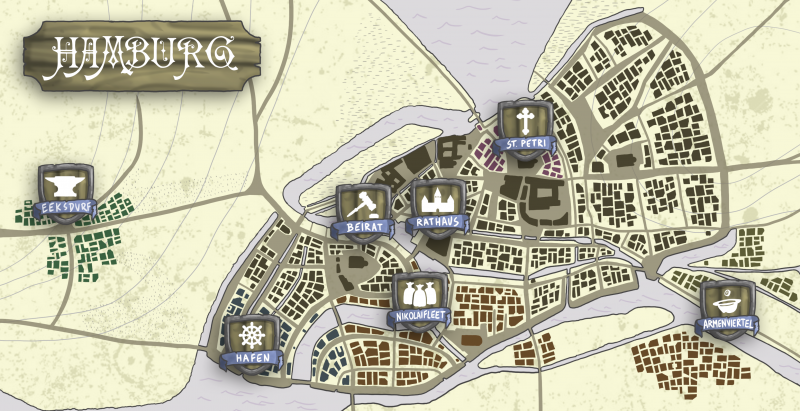
\includegraphics[width=0.8\paperheight,height=\textwidth]{./01-img/map.png}
    \label{fig:map}
	\end{figure}

\end{landscape}
